


\subsection{Basics of Neural Networks}\label{subsection: intro_neural_network}
Neural Networks are models that learn important features and feature associations directly from data. % by training with a portion of the total data. 
These are typically supervised learning models used for classification or regression. They consist of a series of layers of linear combinations of the input data each with real value parameters known as weights and biases, combined with activation functions that enable learning {\it non-linear}, potentially very complex, relationships in the data. The weights tell us the relevance of the input feature with respect to the output, and the biases are the threshold value that determine the output. %(e.g. if a final output value is greater than a certain threshold then is A otherwise is B). 
Fitting these quantities to the data minimizes the %loss These quantities are the ones that guarantees the minimum
loss,
meaning the prediction is as close as possible to the original target/label \citep{nielsen_NN}. For Deep Neural Networks (DNNs), ``deep'' refers to the fact that there are multiple hidden layers, besides the input and output layer.  %that follow a layer structure, where each layer learns new and complex features of the data, architecture of these models usually consist on a input layer + hidden layers + output layer. Each hidden layer has weights and biases that is connected with the other hidden layers and both input and output data. 
With this architecture the features learned by each layer do not follow a human selection, rather, the features arise in the analysis of the data \citep{LeCun_Bengio_Hinton_2015}. Among DNNs, CNN models have layers that represent convolutional filters.
%The layers used in this work are:  \mintinline{c}/Conv2D/, \mintinline{c}/Dropout/, \mintinline{c}/Flatten/, \mintinline{c}/Dense/, etc... - a description of the structure and use of these standard layers can be found in 
More information on DNNs and CNNs can be found in \cite{DBLP:journals/corr/abs-1803-08375, 10.5555/2999134.2999257, Dieleman_2015}, as well as \cite{Gieseke_2017}, among many others.

We used the \texttt{Keras}\footnote{\url{https://keras.io/api/layers/convolution\_layers/convolution2d/}.} implementation of the CNN \citep{chollet2015keras}.




\subsection{DIA and noDIA based models architecture}


The input of our Neural Networks are the horizontally stacked images of size $51 \times 153$ for the \diabased\ model (\diff, \search, \temp), and $51 \times 102$ for \nodia\ model (\search, \temp). For both the \diabased\ model and the \nodia\ model $100,000$ images were used, $80,000$ images for training  and for validation and testing $20,000$ each. The images were selected randomly from the $898,963$ and while certainly training with a larger set can lead to higher accuracy, the amount of images was sufficient for this comparison of \diabased\ and \nodia\ models while being conservative with limited computational resource. The data is composed of $50,183$ images labeled as ``bogus'' and $49,817$ labeled as ``real''. %Each model was tested using $20,000$ divided as  $9922$ ``bogus'' and $10,078$ ``real''.\\

The network architectures used for this work are shown in  \autoref{fig:architecturesCNN}, left panel, for the \diabased\ model, and right  panel for the \nodia\ model. More details about the architecture can be found in \hyperref[sec:appendixb]{Appendix C}. Both architectures follow a similar structure. In designing the neural networks, we started with the \diabased\ model and developed an architecture that would match the performance of \citet{Goldstein_2015}.  With this model in hand, we created a \nodia\ with a similar structure in order to enable direct comparison and measure the effect of the change in the input data. 
We emphasize that in the development of our models we followed two general guidelines: 
\begin{enumerate}
\item We pushed the accuracy of the  \diabased\ CNN model to match the accuracy of \texttt{autoscan}. While a more exhaustive architectural exploration or a hyperparameter grid search may well lead to increased efficacy, matching the accuracy of \texttt{autoscan} (at 97\%) is sufficiently for our demonstration. We further note that this historical data set cannot be further validated (by, for example, assessing the recurrence of transients at a sky position to validate the {\it bogus} nature of a non-simulated detection) and it is subject to potential label inaccuracies that may compromise the ability to achieve a better performance. The final architecture used is one that reached the same accuracy as \citet{Goldstein_2015}, and  False Positive and False Negative Rates most similar to the ones obtain in \citet{Goldstein_2015}  (see \autoref{fig:confusiomatrix_models} and \autoref{sec:results}). Once we matched the \texttt{autoscan} performance, we focused on the potential for removing the \diff\ image from the input.
\item While the architecture of the \diabased\ CNN was designed with the attempt to achieve a specific target performance, the architecture of \nodia\ is deliberately kept as close as possible to that of the \diabased\ model. This enables a direct comparison of the effects of the removal of the \diff\ image. 
In other words, the hyperparameters and architecture of \nodia, shown on the right in \autoref{fig:architecturesCNN} were not optimized explicitly for RB classification, rather we chose a standard architecture, only modifying the original design to adapt for the different dimensionality of the input data. One further deliberate modification is implemented in the choice of a single-filter first layer for \nodia. The CNN that is not offered the \diff\ image needs to learn the image PSF, which is constant across the postage stamp-size image, and can be modeled with a single filter. 
\end{enumerate}

\tatiana{A grid search was implemented in the \nodia\ model, varying the kernel size of the three convolutional layers 1, 3 and 6 and the batch size. %The combination tested and their respective performances are given in APPENDIX. 
No better combination of hyperparameters was found.  }

\tatiana{As part of the optimization tasks, pre-made deep learning models available in \texttt{Keras} were trained with the data of the \diabased\ case presented here. VGG16 \citep{VGG16} was implemented, while the model has a similar performance in terms of accuracy and other metrics, presented overfitting after ~50 epochs. ResNet 50-V2 \citep{RESNET50V2} was also implemented, overfitting was presented during all training process. Pre-made architecture limit the size of the images used for train the model. To implement these architectures the data must have the form of: (height, width, 3). In consequence the selection that we made in this work to horizontally stacked the images is not longer possible, also training the model with the \nodia\ approach is only possible by changing the shape of the images to match the require third depth axis. In such a case we will loss the spatial and geometrical information of the data.   }


\subsection{Saliency maps}\label{subsec: saliency}


% \masao{This is a very interesting section!  For readers like me who don't know much about how saliency maps are produced, can you write a couple of sentences about how they are made?  I think you said something about removing each pixel and looking at how much the predictions change.  A short description is helpful for the uneducated reader like me.}

Saliency maps quantify the importance of each pixel of an image in input to a CNN in the training process. They provide some level of interpretability through a process akin to feature importance analysis by enabling  an assessment of which are the pixels the model relies on the most for the final classification. If the task were, for example, to identify cats and dogs in images, the expectation will be to find that the most important pixels are located within the the dog or cat bodies, and not in the surrounding, while if the task were to identify activities performed by cats and dogs, one may find the important pixels both within the dogs and in the surrounding, particularly in objects associated with the performed tasks. Furthermore, some portion of the subject's body may be most distinctive (ears, nose) and we would expect more importance being given to those pixels. The "importance": of a pixel would be simply measured by the weight the trained NN assigns to that pixel in the case of a single-layer perceptron, but in the case of Deep Neural Networks, a highly non-linear operation is performed on the input data, and the importance, or saliency, of an input feature, or pixel, is harder to assess. We follow \citep{simonyan2014deep}'s definition of saliency: denoting the class score with $S_c$, such that the NN output on image $\mathcal{I}$ is represented by $S_c(\mathcal{I})$, the saliency map is given by :
\begin{eqnarray}
 S_c(\mathcal{I}) \approx w^T \mathcal{I} + b,\\
 w = \frac{\partial S_c}{\partial \mathcal{I}} \biggr\rvert_{\mathcal{I}_0}.
 \end{eqnarray}
 
That is: $w^T$ is the weight and $b$ the bias of the model. $w$ is the derivative of $S_c$ with respect to $\mathcal{I}$ calculated specifically in the local neighborhood of pixel $\mathcal{I}_0$, and the approximation sign indicates a first order Taylor expansion has been used to approximate the solution.
The interpretation of the decision making by the CNNs have been studying as a tool for improving the efficiency of the performance of the CNNs, as done by \citep{DBLP:journals/corr/abs-2105-00937}.\tatiana{Within the transient detection approach, previous works, \eg\  \cite{Reyes_2018}, have implemented Saliency maps to detect the relevant pixels and improve perfomance on transient classification. }


\begin{figure*}
    \centering
    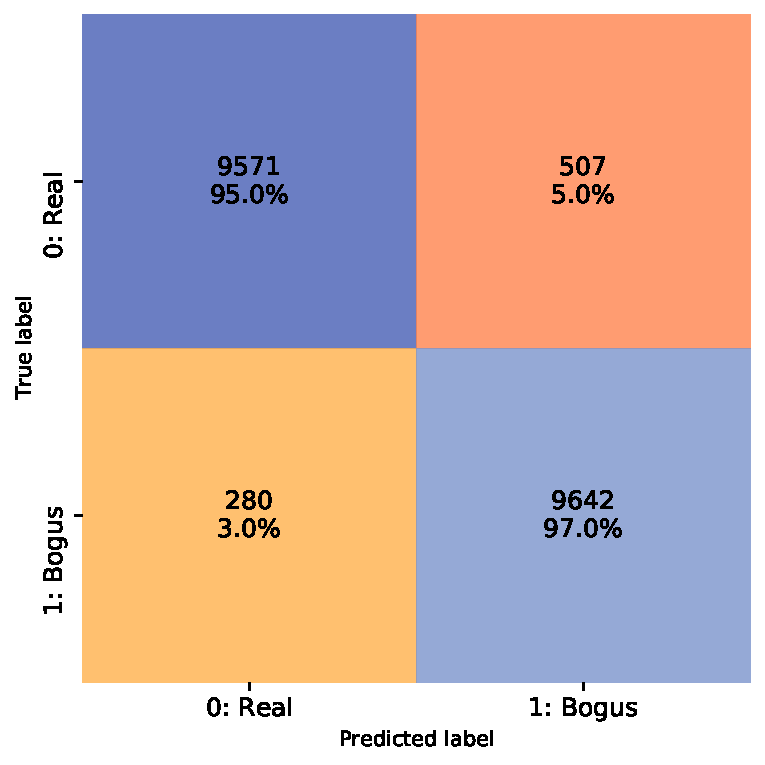
\includegraphics[width=0.45\linewidth]{
    figures/confusionmatrix_model_100K20KNERSCstam0-9CCCC_3s3DH.pdf}
    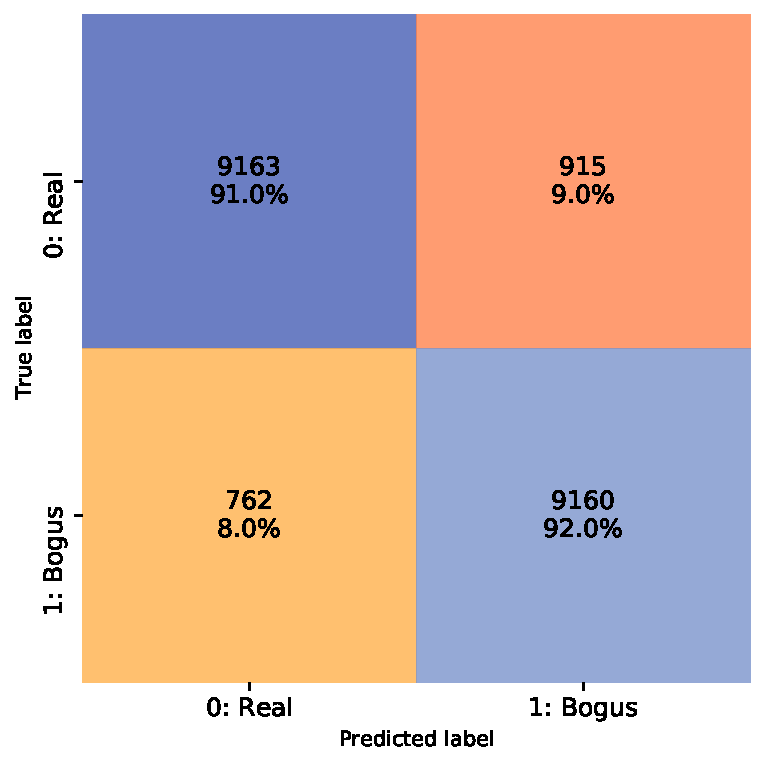
\includegraphics[width=0.45\linewidth]{
    figures/confusionmatrix_model_100K20KNERSCstam0-9CCCC_3s2DH.pdf}
    \caption{Confusion matrix (CM) for our testing data, a set composed of $10,078$ objects labeled as ``real'' and $9,922$ as ``bogus''.  Squares of the matrix, from the top left in the clockwise direction, indicate: True Positive (TP, \texttt{label = 0}, \texttt{prediction = 0} ), False Negative (FN, \texttt{label = 0}, \texttt{prediction = 1}), True Negatives (TN, \texttt{label = 1}, \texttt{prediction = 1}), and False Positive (FP, \texttt{label = 1}, \texttt{prediction = 0}). We note that here, somewhat unusually, 0 corresponds to ``real'' and ``positive'', and 1 to ``bogus'' and ``negative'', as we chose to remain consistent with the original labeling of the data presented in \citep{Goldstein_2015}. 
    {\it Left}: The CM of our \textbf{\diabased } model shows that from the $10,078$ transients labeled as ``real'', $9,571$ (\ie, 95\%) were correctly classified and the accuracy for the TN objects is even higher, at $97\%$. {\it Right}: The CM for the \nodia\ model shows that of the $10,078$ transients labeled as ``real'', $9,163$ (\ie, 91\%) were predicted correctly and the TN accuracy is $92\%$. }
    \label{fig:confusiomatrix_models}
% \end{figure}
\end{figure*}


\begin{figure}
    \centering
    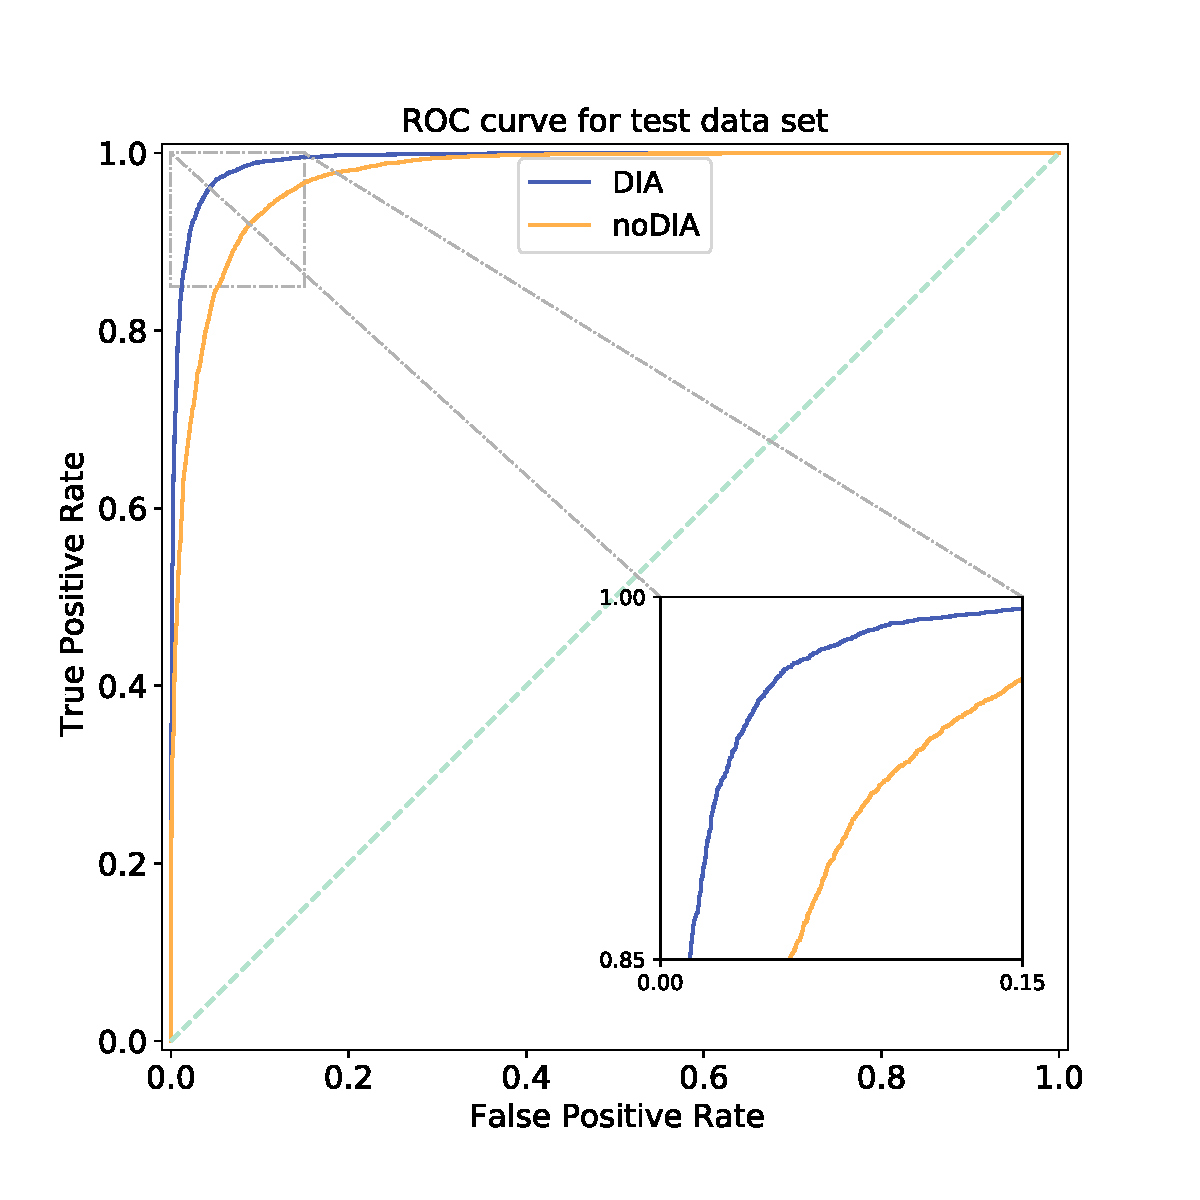
\includegraphics[width=1\linewidth]{
    figures/ROC_zoom.pdf}
    \caption{ROC curve for the $20,000$ images used for testing, Blue line for the  \diabased\ model, the area under the curve is $0.992$. Orange line, for the \nodia\ model, the area under the curve is $0.973$. This figure is discussed in \autoref{sec:results}.}
    \label{fig:roc_models}
\end{figure}

\begin{figure*}
    \centering
    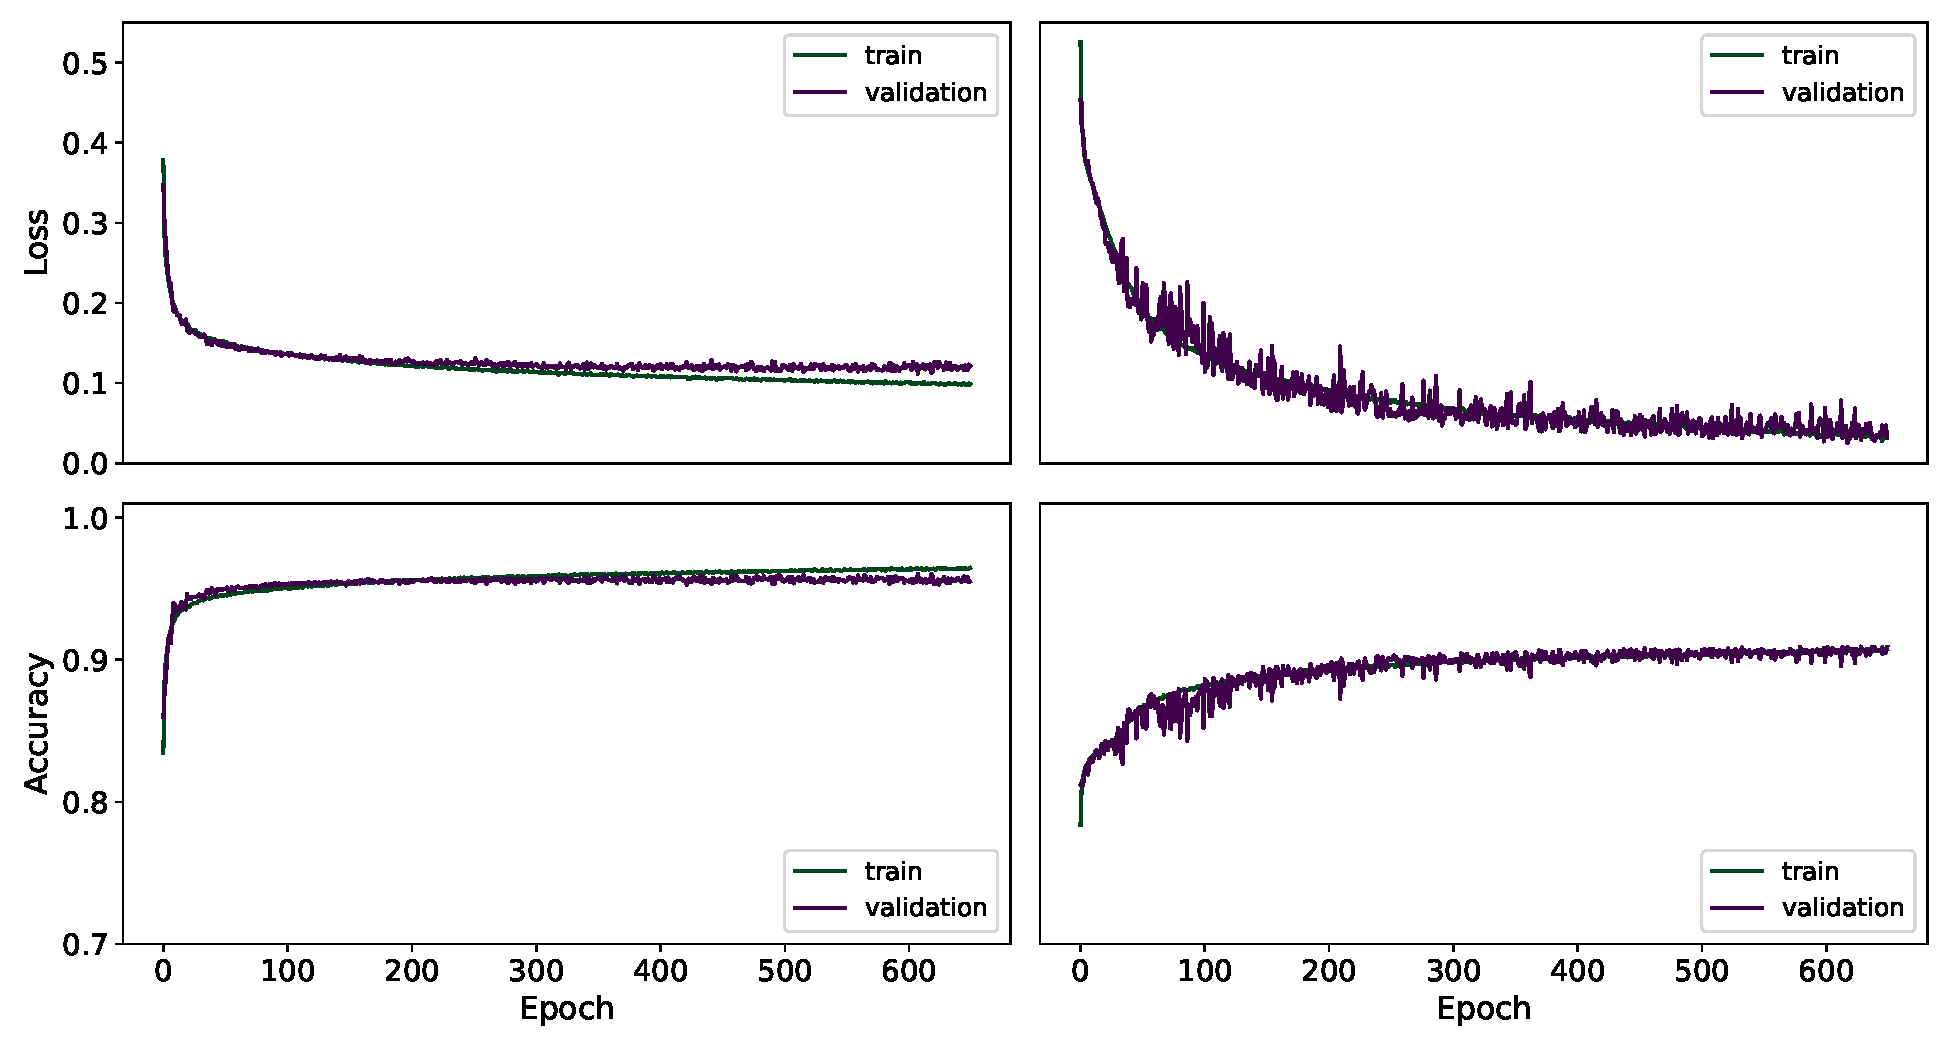
\includegraphics[width=0.9\linewidth]{
    figures/losscc.pdf}
    % \includegraphics[width=0.49\linewidth]{
    % figures/lossacc_modeloverleafCCC_scale(1).pdf}
    \caption{Loss (top) and accuracy (bottom) for both models presented in this work. Purple lines correspond to the validation data (20\% or 20,000 images) and green to the training data (80\% or 80,000 images). {\it Left}:  results for our \diabased\ model  (\autoref{fig:architecturesCNN}). {\it Right}: results for the \nodia\ model (\autoref{fig:architecturesCNN}). %This figure is discussed in \autoref{sec:results}.
    }
    \label{fig:loss_models}
% \end{figure}
\end{figure*}
Each pixel in an image in the training set is associated with the corresponding pixel in the saliency map, and the saliency score (the importance) of that pixel measures the change in model output as a function of changes in the value of that input pixel by back-propagation. The higher the value of a pixel in a saliency map, the more influence that pixel has in the final classification. In this work we also refer to these maps as maps of pixel importance. 


In our case, given the side-by-side organization of the three elements of the input image set, %(\diff, \search, \temp), 
the saliency maps can help us assess how much the \diabased\ model relied on the \diff\ to enable correct classification, and, thus, provide some intuition in the difficulty of the challenge offered to the \nodia\ model. 


For the \diabased\ model we have an expectation guided by intuition: that a greater concentration of important pixels should be found in the \diff\ image. In \autoref{sec:results},  we will consider the veracity of this hypothesis both qualitatively by visually inspecting the saliency maps, and by designing a saliency-based metric that enables a quantitative approach. We calculated the normalized sum of the saliency pixel values for each third of the image-triplet, corresponding to \diff, \search, \temp:

\begin{eqnarray}
\begin{split}
\idiff=\frac{\sum_{p_d}{s_{p_d}}} {\sum_{p}{s_p}};\\
\isearch=\frac{\sum_{p_s}{s_{p_s}}} {\sum_{p}{s_p}};\\
\itempl=\frac{\sum_{p_t}{s_{p_t}}} {\sum_{p}{s_p}};
\label{eq: saliencymetric}
\end{split}
\end{eqnarray} 
where $I$ indicated the importance of a segment of the input image, $p$ is an index running over all pixels and $s_p$ indicates the value of pixel $p$ in the saliency map. The denominator normalizes each metric by the total sum of the saliency pixel values. In the numerators, $p_d$ denotes the pixels in the leftmost third of the image, corresponding to \diff; $p_s$ the middle third corresponding to the \search; and $p_t$ the right most third, corresponding to the \temp. 
This metric allows us to assess the relative importance of the \diff\ (\search\ or \temp) component of the image in performing RB classification. Results from these metrics are discussed in detail in \autoref{subsec:results_seliancy}.\\

% This study is reproducible and all the code that supports the analysis presented here is available on a dedicated \texttt{GitHub} repository. \footnote{\url{https://github.com/taceroc/DIA_noDIA}.}



%\begin{figure*}
%\begin{tabular}
%\begin{minipage}[b]{0.45\linewidth}
%%\begin{figure}[t!]
%    \centering
%    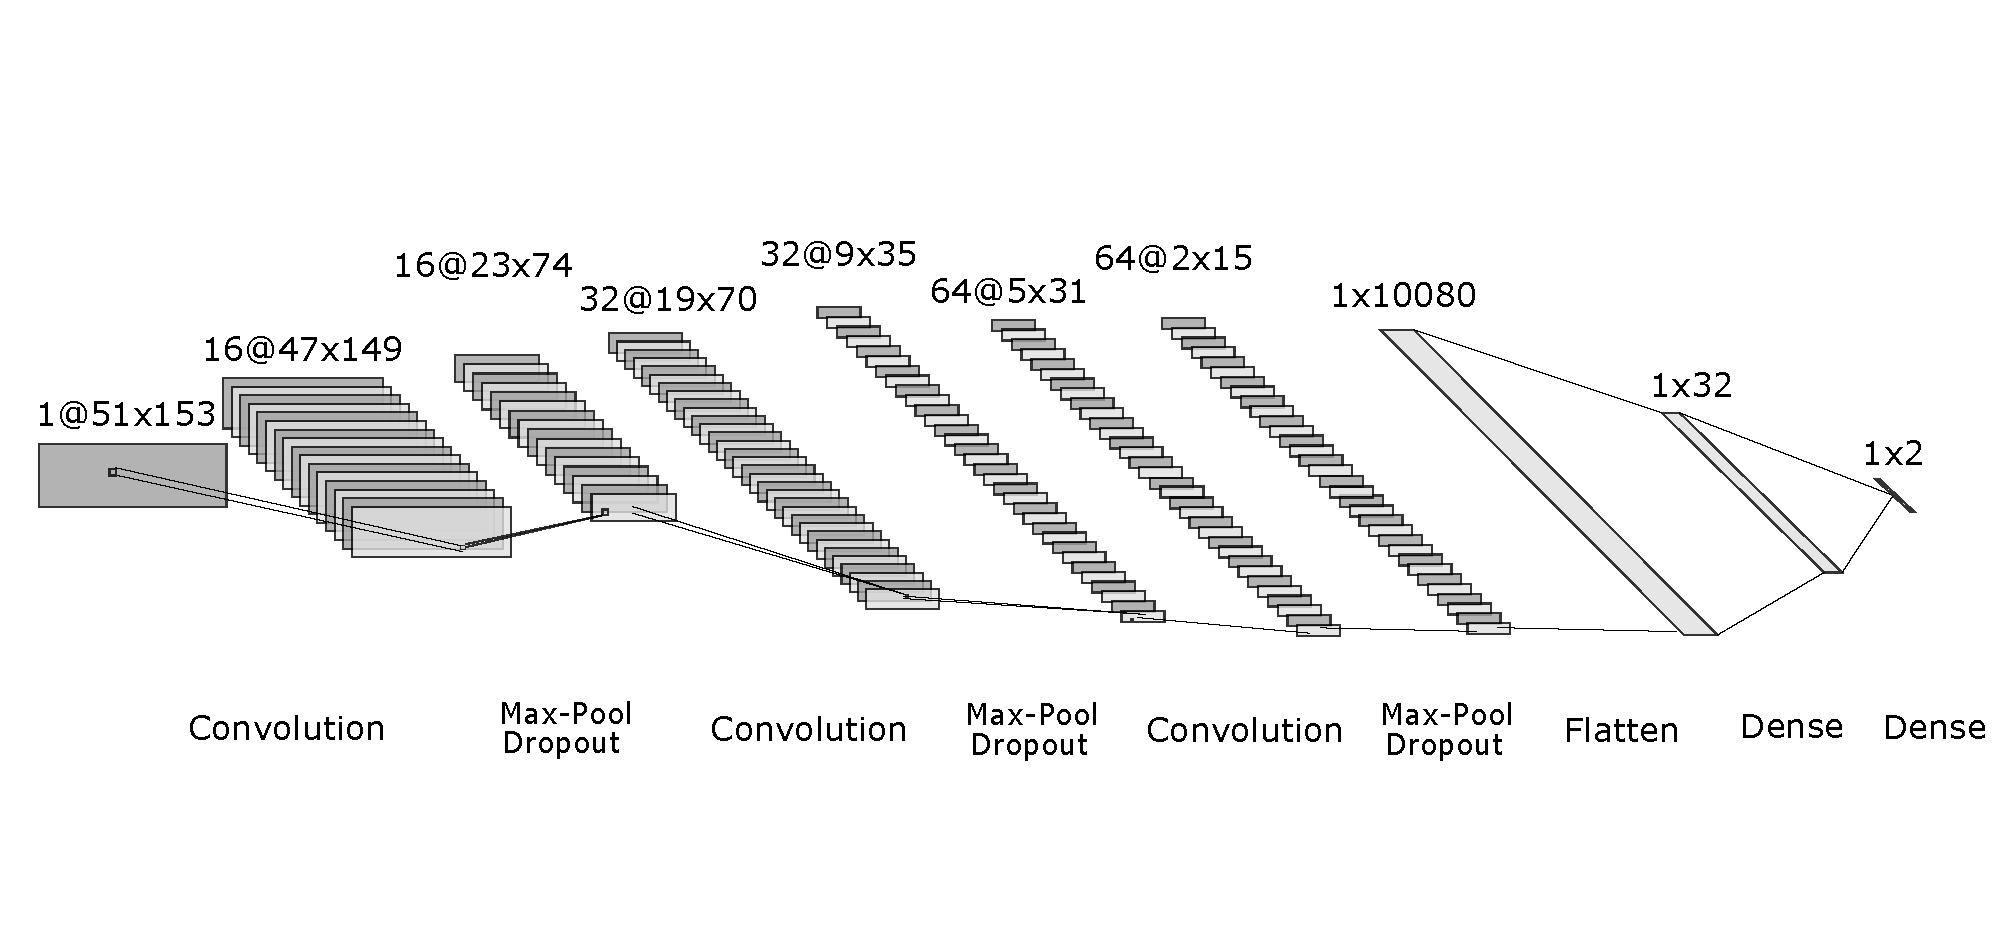
\includegraphics[width=0.8\linewidth]{
%    figures/aaa_big.pdf}
%    \caption{Architecture of the Neural Network used in this project to classify ``real'' and ``bogus'' transients from the image triplet \textbf{(\diabased\ model)}. The input layer was $51 \times 153$ (see left \autoref{fig:examples_hstack_normalization}); a convolution layer $(5\times 5)$ learned $16$ filters; max pooling $(2\times2)$ and dropout; convolution $(5\times 5)$ learned $32$ filters;  maximum pooling $(2\times2)$ and dropout; convolution $(5\times 5)$ learned $64$ filters;  maximum pooling $(2\times2)$ and dropout; flatten layer, Dense $(32)$ and the output was a Dense $(2)$-class layer. The illustration was made using NN-SVG tool by \cite{LeNail2019}.}
%    \label{fig:architecture_NN}
%\end{minipage}
%\begin{minipage}[b]{.45\textwidth}
%%\begin{figure}[t!]
%    \centering
%    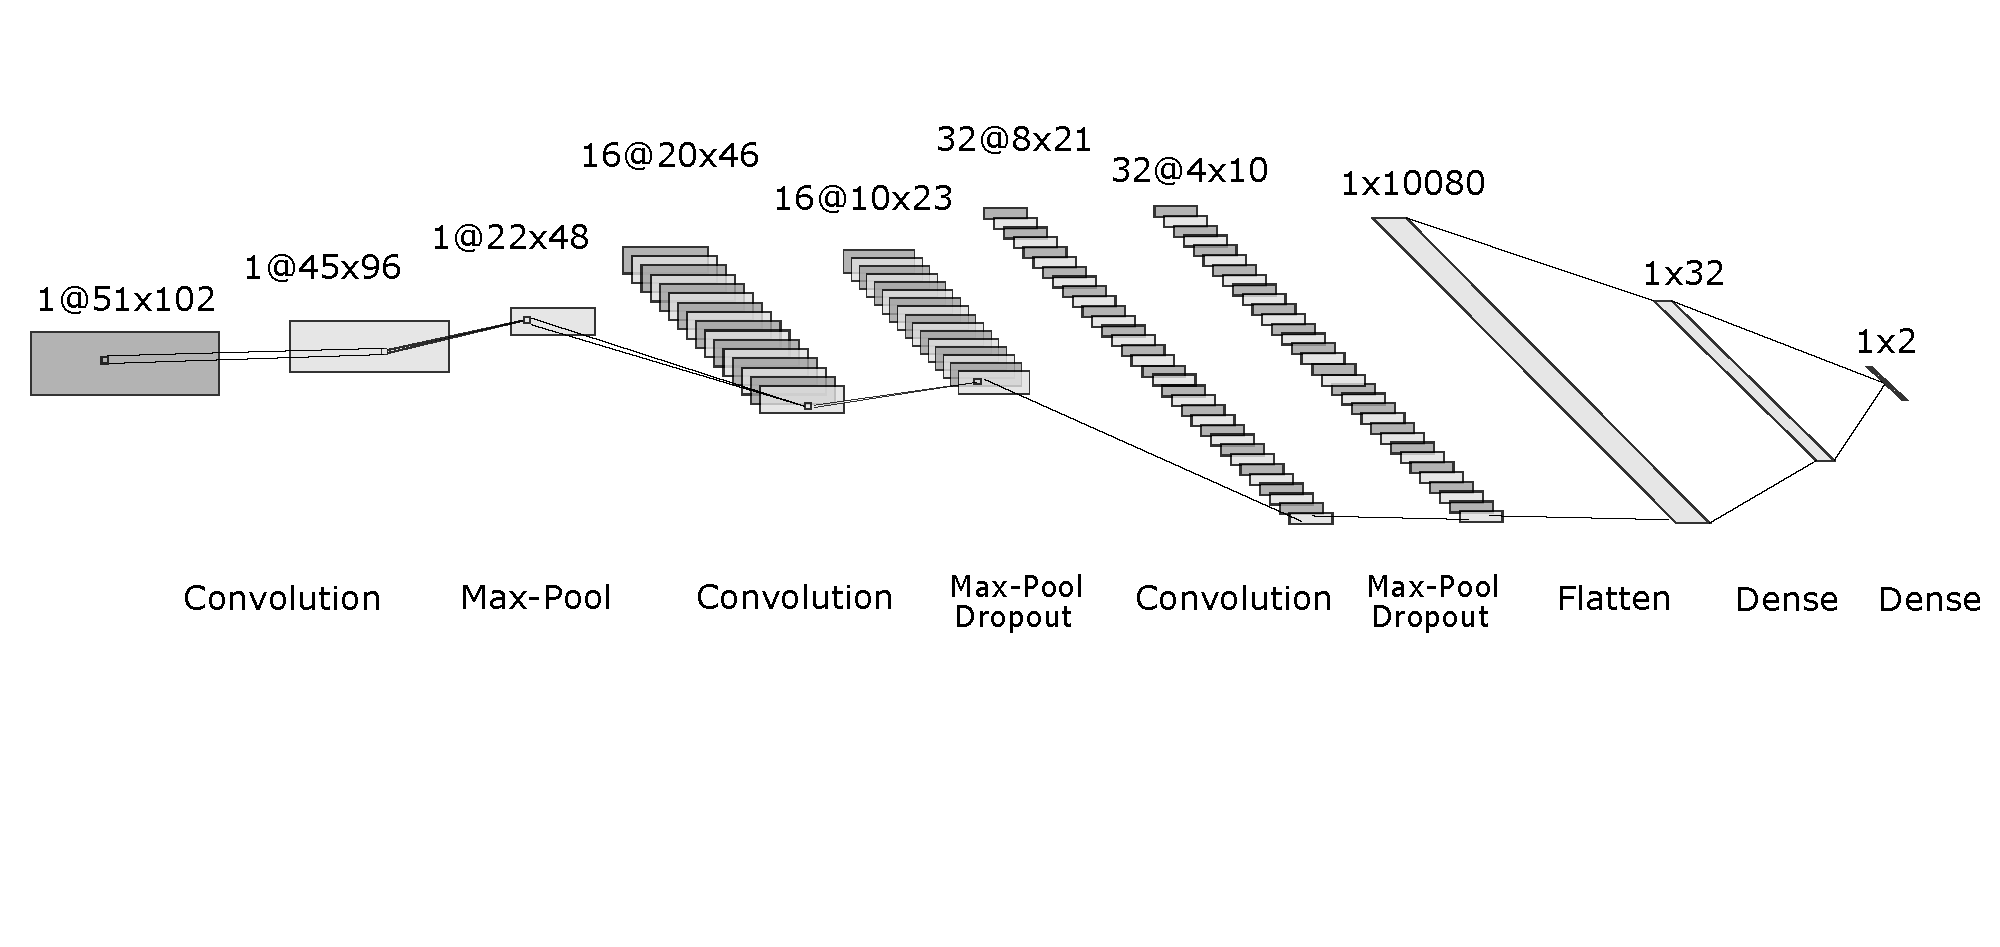
\includegraphics[width=0.8\linewidth]{
%    figures/ccc_bug.pdf}
%    \caption{Architecture of the Neural Network used in this project to classify ``real'' and ``bogus'' transients from the image duplex \textbf{(\nodia\ model)}. The input layer was $51 \times 102$ (see right \autoref{fig:examples_hstack_normalization}); a convolution layer $(7\times 7)$ learned $1$ filter; maximum pooling $(2\times2)$; convolution $(3\times 3)$ learned $16$ filters;  maximum pooling $(2\times2)$ and dropout; convolution $(3\times 3)$ learned $32$ filters;  maximum pooling $(2\times2)$ and dropout; flatten layer, Dense $(32)$ and the output was a Dense $(2)$-class layer.
        %\footnotetext{$\dag$ 
%        {The illustration was made using NN-SVG tool by \cite{LeNail2019}.}
%        }
%    \label{fig:architecture_2DNN}
    
%\end{minipage}
%\end{tabular}{cc}
%\end{figure*}

% \begin{figure}[hbt!]
%     \centering
%     \includegraphics[width=0.9\linewidth]{
%     figures/CNN.pdf}
%     \caption{Architecture of the Neural Network used in this project to classify ``real'' and ````bogus'''' transients from the image triplet. The input layer is $51 \times 153$ (see \autoref{fig:examples_hstack_normalization}; a convolution layer $(5\times 5)$ learns $16$ filters; maximum pooling $(2\times2)$; convolution $(5\times 5)$ learns $32$ filters;  maximum pooling $(2\times2)$; flatten layer, Dense $(32)$ and the output is a Dense $(2)$-class layer.}
%     \label{fig:architecture_NN}
% \end{figure}




% The first convolutional layer of this model, intends to recover the PSF (Point Spread Function) of the 
% \begin{itemize}
% \item \mintinline{c}/Conv2D/:\\

% According to the documentation of Convolutional layers in \url{https://keras.io/api/layers/convolution\_layers/convolution2d/}. The first parameter (\mintinline{c}/filter = 16 or 32 /) refers to the number of filters that the layer is going to learn. The outer layers learn less from the data than the inner layers. The second parameter (\mintinline{c}/kernel_size = (5,5)/) refers to the width and height of the filter that is multiplying the input data, the elements of the filter are the weights. The third parameter (\mintinline{c}/padding = "valid"/) define the way that the filter is going to sweep the input data, \mintinline{c}/"valid"/ refers that the operation between filter and input data is possible only if all the elements of the filters have a corresponding element in the input data. With this parameter the size of the output data is going to be smaller than the input. The latter parameters used here is the \mintinline{c}/activation = "relu"/, ``Rectified Linear Unit''. The output data, know as feature map, is pass through the activation function to get the bias. The \mintinline{c}/"relu"/ function is defined as:
% \begin{equation*}
% ReLU = 
% \begin{cases}
%     0, & x\le0\\
%     x, & x>0
% \end{cases}
% \end{equation*}
% The ReLU is an efficient activation function that improves the performance of the Neural Network. [\cite{DBLP:journals/corr/abs-1803-08375, 10.5555/2999134.2999257}]

% \item \mintinline{c}/MaxPooling2D/:\\
% Reduces the size of the output given in \mintinline{c}/Conv2D/ by a factor of $2$, selecting maximums values.

% \item \mintinline{c}/Flatten/:\\
% Reduces the dimensions of the data to be a one dimension array.

% \item \mintinline{c}/Dense/:
% Make the previous layer all fully connected with the next layer.\\
% \end{itemize}






% %A optimizer, loss and metric:
% \begin{minted}{python}
% opt = keras.optimizers.SGD(learning_rate=0.01)
% model.compile(optimizer=opt, loss="sparse_categorical_crossentropy", metrics=["accuracy"])
% \end{minted}

% The model is fit to the training data and this is split to have a validation set. We use \mintinline{c}/epochs=50, batch_size=20/.
% %and fitting the model as:
% \begin{minted}{python}
% history = model.fit(feat_tr2, targ_tr, validation_split=0.20, epochs=50, batch_size=20)
% \end{minted}

% The training data is divided into groups of $20$ elements. The weights of the model are updated after each group of $20$ is been fitted. After the $1$st epoch, the weights have been updating the numbers of groups of $20$ that exist.\\
